\section{Results}\label{sec:results}
In this section we report the results for our baseline and different configurations for finding utterance embeddings.
Also we present some analysis of our distributional representations.

\subsection{Baseline}
As a baseline we represent each utterance as a bag of words.
We represent each utterance as a sparse vector, were every dimension maps to a word in the vocabulary.
We then train a Naive Bayes model and a K-Nearest Neighbor classifier on the dialog act tagging task, both for the full tag set of 42 tags as well as on the aggregated tag set of 8 tags.
The results can be seen in Table \david{make table with results} and \david{a seperate table for aggregated tag set pherhaps?} respectively. \david{Report best baseline explicitly here}.
Furthermore we calculate a trivial baseline where every utterance is classified as the most frequent dialog act tag, this would result in an accuracy of $31.47\%$.

\begin{table}[h]
	\centering

	\begin{tabular}{l|r}
		& \textbf{Accuracy} \\ \hline
		\newcite{kalchbrenner} & 73.9 \%           \\
		\newcite{stolcke2000}  & 71.0 \%           \\
		\newcite{milajevs}     & 63.9 \%          
	\end{tabular}
		\caption{Accuracy scores from other work}
		\label{tab:sota}
\end{table}

\subsection{Classification using Utterance Embeddings}
\david{Do we want to present everything here or just the best?}
We found embeddings for utterances as discussed in section \ref{sec:utt2vec}.
Different setting were used to find these embeddings, we varied the training data, number of training epochs and whether or not we used pretrained word embeddings.
With these utterance embeddings we trained Naive Bayes, K-Nearest Neighbor and Multilayer Perceptron classifiers.
In Table \david{make table} the results for the full tagset are presented, where Table \david{also make that table}, present the results on the aggregated tag set. \david{Report best result here}

\begin{table}[]
\centering
\small
\begin{tabular}{llll|lll}
                   & \multicolumn{3}{c|}{full tagset} & \multicolumn{3}{c}{agg. tagset} \\
                   & NB      & KNN     & MLP     & NB     & KNN     & MLP     \\
\hline
SWDA               &         &         &         &        &         &         \\
SWDA+BNC         &         &         &         &        &         &         \\
\end{tabular}
\caption{Example results table no context. And we need the same table for context.}
\label{tab:results}
\end{table}


\subsection{Using context}
To use the contextual information of the dialog to classify dialog act tags, we experimented with two \david{naive} approaches. We either concatenated or added the embedding of the previous utterance to the embedding of the considered utterance.
The first approach nicely represents the sequentiality of the dialog but it doubles the amount of features for the classifier to consider.
The latter approach is not affected by this curse of dimensionality, however it does lose all sequential information present in the dialog.
The results for both approaches can be seen in Table \david{make table}. \david{Also here, best result in text}

\subsection{Error Analysis}
Utterance embeddings have the property of encapsulating the meaning of utterances from the words that compose them; as with the case of word embeddings, these representations present appealing relations from which similar words (in a semantic sense) appear close by in the high dimension space.
We extract samples from the SWDA corpus belonging to tags that are clearly unrelated, and apply dimensionality reduction to their vector representations using Principal Component Analysis (PCA).
We plot the results in two and three dimensions.
The sampled utterances belong to the following categories: \emph{Wh-question}, \emph{Thanking}, \emph{Reject}, and \emph{Apology}.
Considering the words that are used in these kind of units, sample points should be clearly separated.
The utterance embeddings were extracted using a 300-dimensional model trained on the SWDA corpus using pretrained word vectors.
Figure~\ref{fig:2d_pca} and Figure~\ref{fig:3d_pca} show scatter diagrams of the utterance embeddings after applying PCA.

\begin{figure}
\centering
\begin{minipage}{.23\textwidth}
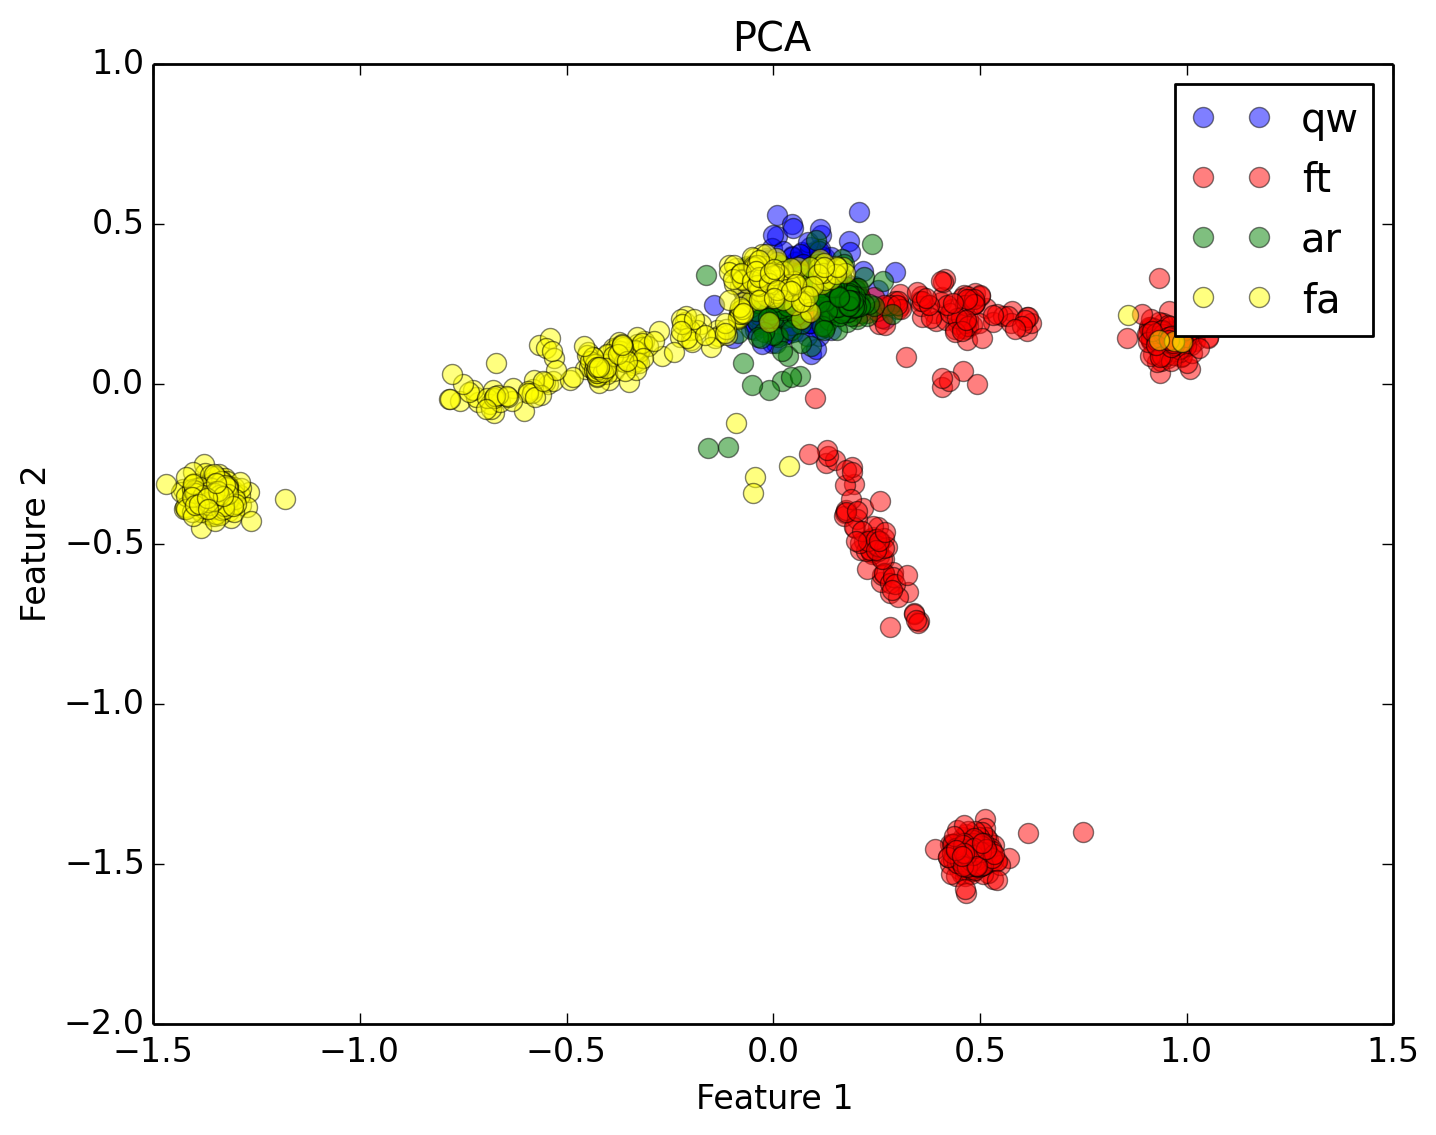
\includegraphics[width=1\textwidth]{img/easy_pca_2d}
\caption{2D PCA.}
\label{fig:2d_pca}
\end{minipage}
\begin{minipage}{.23\textwidth}
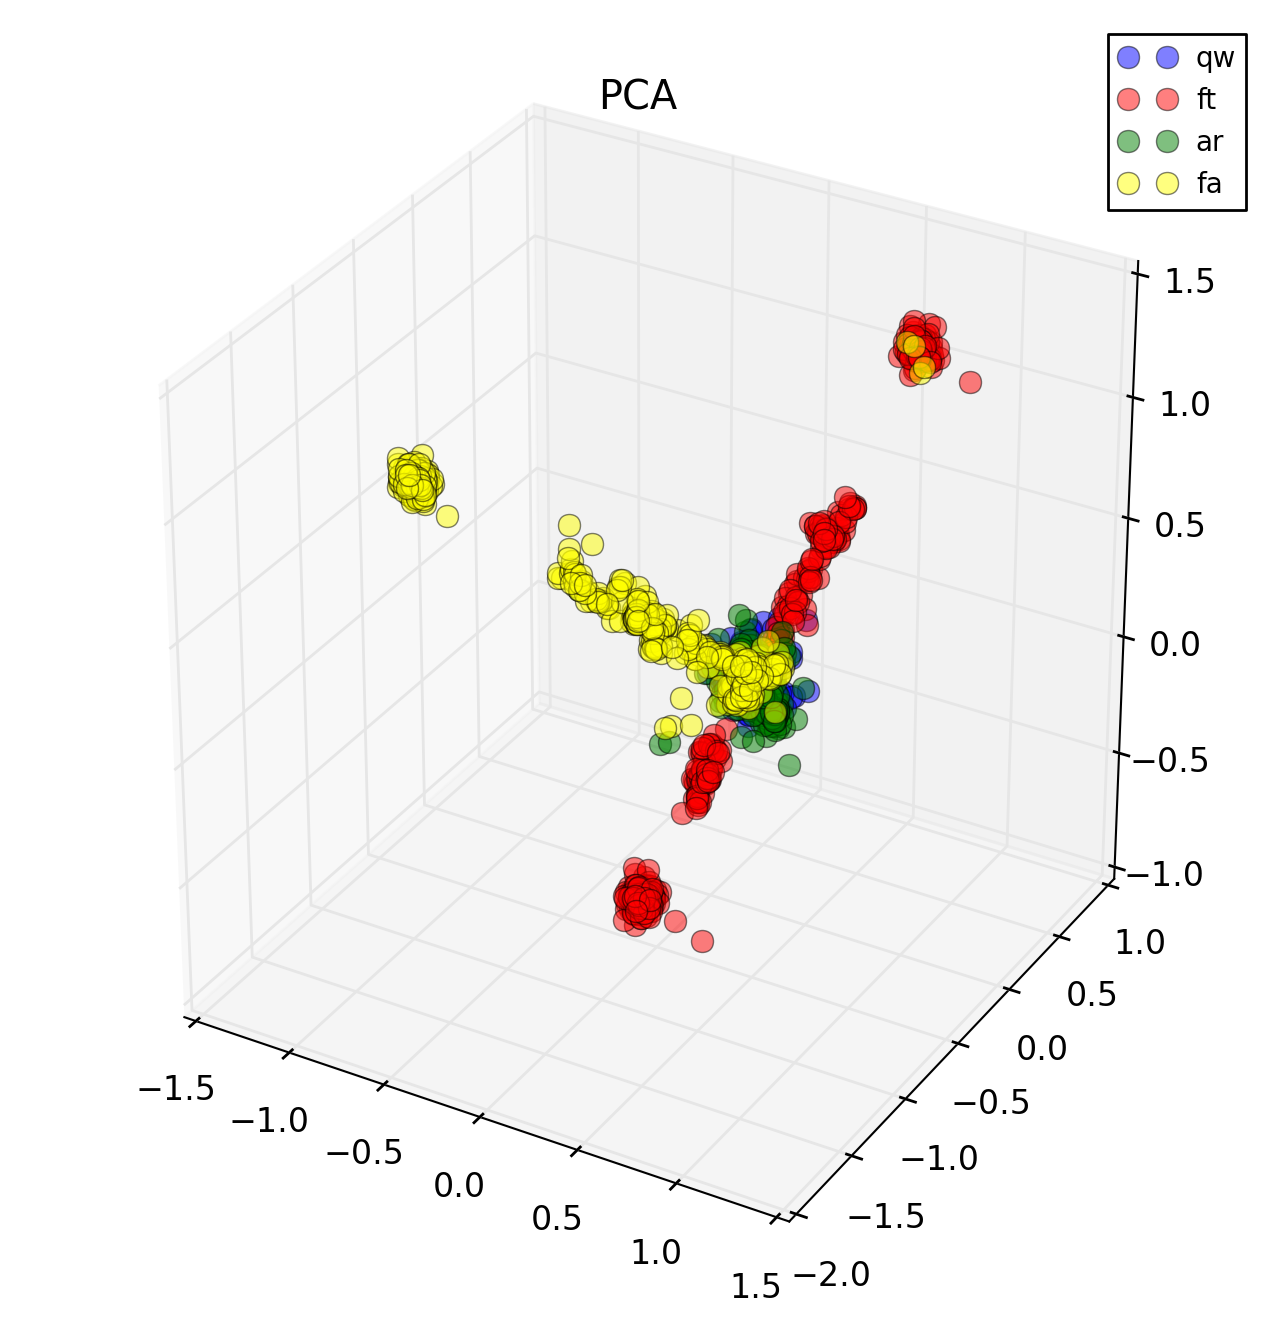
\includegraphics[width=1\textwidth]{img/easy_pca_3d}
\caption{3D PCA.}
\label{fig:3d_pca}
\end{minipage}
\end{figure}

Though, the classification task seems easy considering the previous tag examples, it gets more complicated when we handle other types of utterances.
Figure~\ref{fig:2d_pca} and Figure~\ref{fig:3d_pca} show the scatter diagram after applying PCA to utterance embedding of the five most frequent tags (\emph{Statement-non-opinion}, \emph{Acknowledge}, \emph{Statement-opinion}, \emph{Accept}, \emph{Turn exit}), which account for $78\%$ of the corpus.

\begin{figure}
\centering
\begin{minipage}{.23\textwidth}
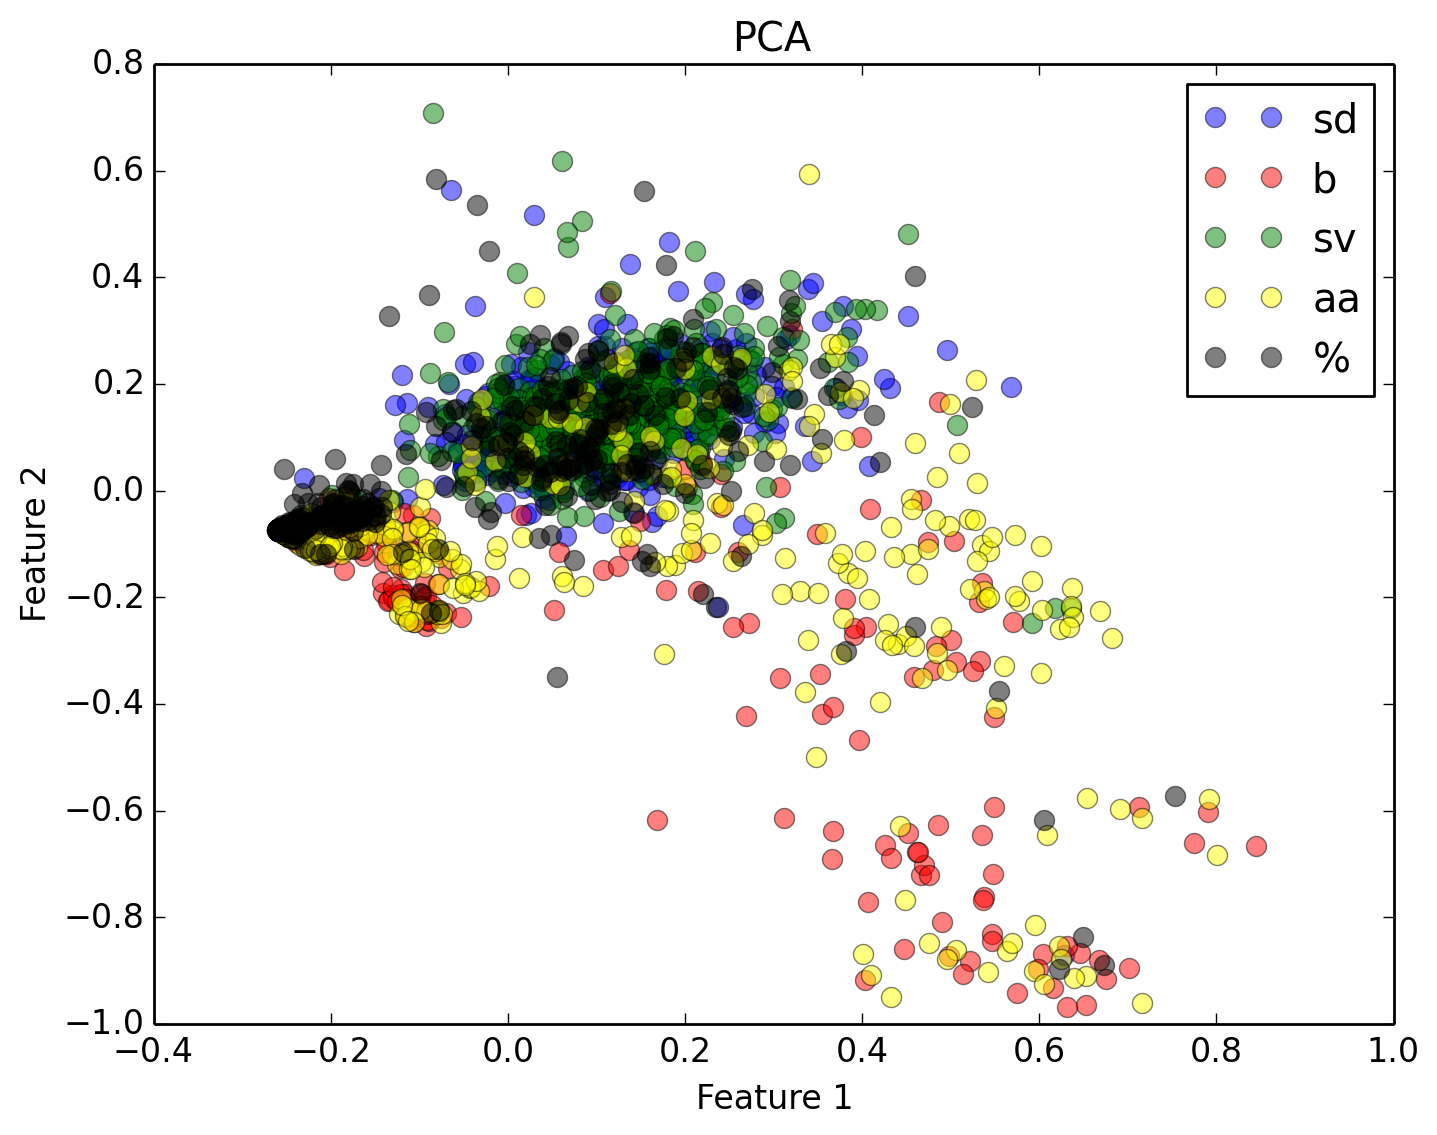
\includegraphics[width=1\textwidth]{img/complex_pca_2d}
\caption{2D PCA.}
\label{fig:2d_pca}
\end{minipage}
\begin{minipage}{.23\textwidth}
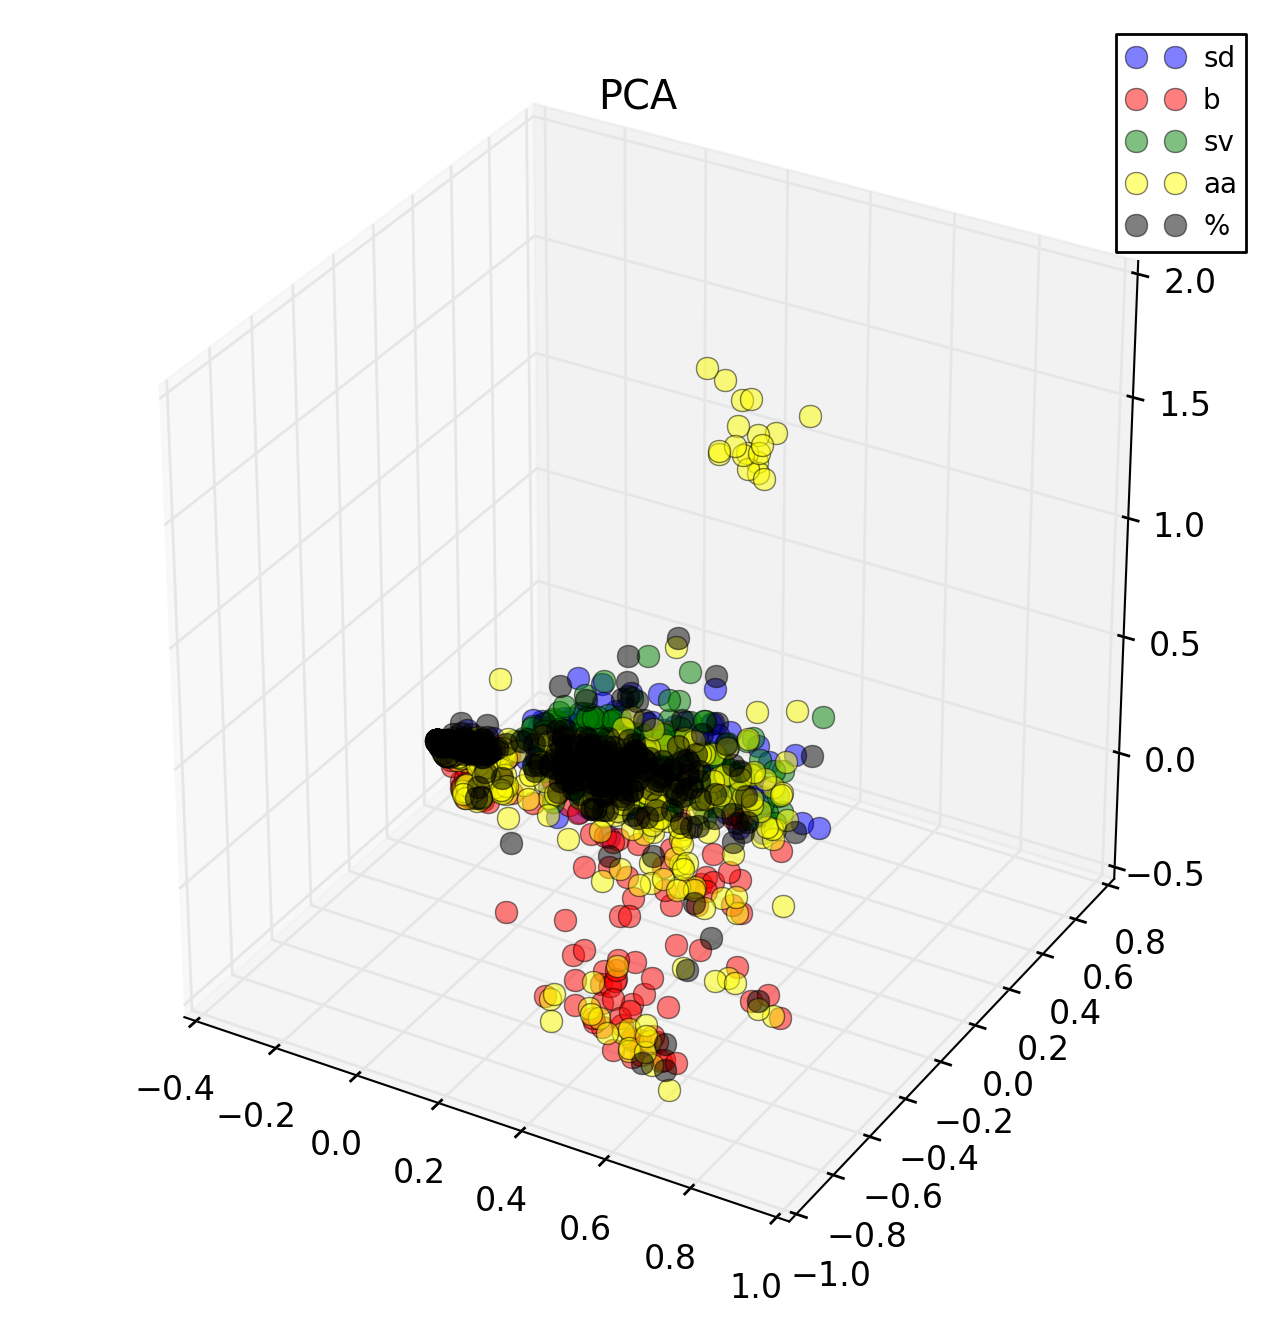
\includegraphics[width=1\textwidth]{img/complex_pca_3d}
\caption{3D PCA.}
\label{fig:3d_pca}
\end{minipage}
\end{figure}
